\chapter{Grundlagen}

\section{Roboter-Mensch-Kollaboration}
\label{sec:roboter-mensch-kollaboration_gru}

Man unterscheidet die Arbeiten mit einem Roboter unter mehrere Arten.
Roboter die mit anderen Robotern gleichzeitig arbeiten nennt man Kooperation zwischen Robotern.
Der Mensch ist in diesem Arbeitsumfeld nicht dabei und kann nur von außen Einfluss nehmen.
\\\\
Als nächstes gibt es die Kollaboration zwischen dem Roboter und dem Mensch.
Hier wird auch eine Unterteilung vorgenommen die unterschiedliche Richtlinien erfordern.

\begin{itemize}
\item Sicherheitshalt, wenn der Mensch den Kollaborationsraum betritt
\item Dauerhafte Überwachung des Abstands zwischen Mensch und Roboter, der mit reduzierter Geschwindigkeit arbeitet
\item Verminderte Geschwindigkeit Führung des Roboters durch den Mensch. Sensoren erfassen die Kräfte, die vom Menschen ausgeführt werden und übertragen sie auf den Roboter
\item Beschränkung der im Roboter ausgeführten Energie \& Überwachung des Roboters auf Kollision und sofortigem Stopp
\end{itemize}

\subsection{Richtlinien}
\label{kol_richtlinien_gru}

In so gut wie allen fällen sind Roboter in der Industrie in einem extra abgesicherten Bereich umzäunt, damit kein Arbeiter sich verletzen kann. Diese Roboter sind umhaust. Es ist nicht möglich in einem gemeinsamen Arbeitsbereich zu kollaborieren.
Damit Menschen im Arbeitsbereich vom Robotern Arbeiten dürfen müssen diese Roboter bestimmte Sicherheitsrichtlinien entsprechen.
Der Roboter darf unter keinen Umständen eine Lebensbedrohliche Gefahr darstellen. Die Norm \ac{ISO} 10218

\section{UR5 Roboter}
\label{sec:ur_robot_gru}

Die Dänische Firma Universal Robots hat den leichten UR5 und mittelgroßen UR10 Roboter hergestellt mit den erfüllbaren Normen, um mit diesem Roboter zu kollaborieren. Man kann sich im laufenden Betrieb in der Nähe aufhalten um Wegpunkte zu \ac{teachen} oder auch gleichzeitig an einem Werkstück zu arbeiten.
Im Folgenden Kapitel werden die Eigenschaften des UR5 Roboters erörtert.

\subsection{Kinematik}
\label{ur_eigenschaften_gru}

\begin{figure}[H]
  \centering
    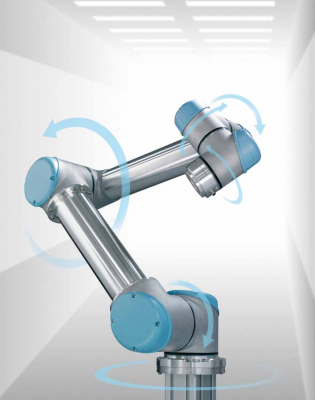
\includegraphics[width=0.6\textwidth]{pic/ur5_robot.png}
      \caption[UR5 Roboter]{Abbildung zeigt den UR5 Roboter von universal Robots}
      \label{fig:schnittstellen_schichten}
\end{figure}

Der Roboter besitzt 6 Gelenke die ihm ermöglichen einen 360° Arbeitsbereich mit einem Radius von ca. 85 cm zu ermöglichen. Gesteuert wird er von einem Linux Rechner, der sich in der Nähe befindet.
Die Festplatte für das System ist eine Speicherkarte, die leicht ausgetauscht werden kann.
\\\\
Um den Rechner anzusprechen existiert bei lieferung ein Touch Tablet, das für das Linux System den Visuellen Output gibt. Beim starten des Systems wird auch automatisch die Software für den Roboter gestartet. Die Software nennt sich Polyscope und wurde in Java geschrieben. Diese Software verbindet sich per TCP/IP auf den \ref{URControl}. Ein Server Programm das die Schnittstelle von dem Linux System zu dem Roboter Controller auf dem Rechner Herstellt.
\\\\
Die Polyscope Software läuft im normalen Modus und den Administrativen Modus. Der Normale Modus ermöglicht es Programme zu erstellen, laufen zu lassen und Grundeinstellungen vorzunehmen. Außerdem kann ein Software Update der Polyscope Software gemacht werden.

\subsection{Peripherie}
\label{sub:ur_update_gru}

Zwei Arten von Updates sind hier zu unterscheiden. Zum einen kann das Linux System geupdatet werden. Auf normalem wege über den Packetmanager des Systems, oder wenn man das neuste Image von Universal Robots runterläd und dann das System neu aufspielt. Hier ist jedoch zu beachten, dass dabei alle Daten verloren gegangen werden. Deshalb sollte eine Datensicherung vorgenommen werden. Wie dies geschieht wird im darauf folgenden Unterkapitel beschrieben(\ref{ur_datensicherung_gru}).
\\\\
Updates für dem Roboter müssen allerdings manuell gemacht werden. Hierfür müssen die aktuellen Updates von der Homepage von Universal Robots runtergeladen werden. Die Update-Datei muss mit der dateiendung .urup auf einen USB Stick mit einem FAT32 Dateisystem abgelegt werden.\\\\
Nachdem der USB Stick an das Linuy System angeschlossen ist, kann von der Polyscope Software das Update ausgeführt werden. Einstellungen->Updates.\\
Im Administrativen Modus können nach dem Update die Firmware's der einzelnen Gelenkcontroller geupdatet werden. Die werden im Update mitgeliefert. Die einzelnen Schritte sind in den Dokumentationen beiliegend auf der CD zu finden.

\subsection{Datensicherung}
\label{sub:ur_datensicherung_gru}

Die Daten des Roboters sind abgelegt in root verzeichniss unter 

\begin{lstlisting}[caption={Pfade Der UR5 Relevanten Dateien}, label=lst:ur5data ,captionpos=b] 
/root/.urcontrol    #Konfigurationsdateien des Ur5Roboters
/programs   		#alle geschriebenen Programme unter Polyscope
\end{lstlisting}

Es ist möglich die Dateien per USB Stick zu sichern oder über Programme wie ``SCP'' über das Netzwerk zu Kopieren.

\section{Programmierschnittstellen vom UR5}
\label{sec:programm_api_uebersicht_gru}

Der Ur5 Roboter kann auf drei Ebenen angesprochen werden.\\

\begin{itemize}
\item Polyscope
\item URScript
\item C-Api
\end{itemize}

In dieser Arbeit wird versucht über alle Ebenen den Roboten Roboter anzusprechen. 
Es wird außerdem aufbauend auf URScript ein eigener Adapter entwickelt, um eine neue Möglichkeit zu untersuchen, um den Roboter anzusteuern.
Der Adapter wird für die Programmiersprache Python entwickelt. Gründe hierfür werden im Kapitel für diese Schnittstelle erörtert(siehe \ref{sec:urscript_adapter})

\begin{figure}[H]
  \centering
    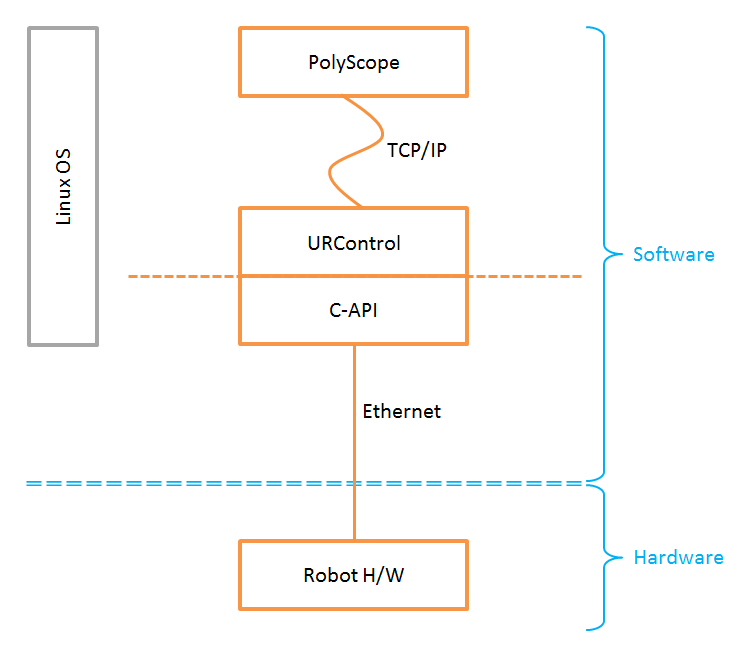
\includegraphics[width=0.8\textwidth]{pic/ur_programming_levels.png}
      \caption[Schichten der Software Schnittstellen]{Übersicht über die
      Schichten der bestehenden Software Schnittstellen des Ur5 Roboters}
      \label{fig:schnittstellen_schichten}
\end{figure}

\subsection{Kriterien für die Bewertung der Schnittstellen}
\label{sub:criterias_of_solutions_kon}

Die Schnittstellen werden wie folgt bewertet:

\begin{itemize}
\item Programmierbarkeit
\item Interaktion mit Programm,
\item Möglichkeit zu Debuggen und Testbarkeit
\item Aufwendung
\end{itemize}

Wie schwer ist es ein Programm für die einzelnen Schnittsellen zu entwickeln.
Kann der Mensch das Programm Intuitiv bedienen? Wichtig hierbei ist, dass der Mensch mit dem Roboter Kommunizieren kann. Dies geschieht am besten, wenn der Mensch nicht Kryptisch was eingeben muss. Der Mensch braucht Anwenderfreundliche Programme.
\\\\
Beim Entwickeln von Programmen ist es wichtig, dass der Entwickler Fehler im Programm entdeckt um diese schnell zu beheben.
Je Größer und Komplexer das Programm wird, desto schwieriger wird es Fehler zu entdecken.

\section{URControl}
\label{sec:ur_control_gru}

Der URController eine Server Anwendung die auf dem Rechner des Roboters läuft. 
Dieser Controller dient als Schnittstelle von der Roboter Hardware und der Software die den Roboter ansteuern wollen. 

\subsection{Konfiguration des URControllers}
\label{urcontrol_rci_gru}

Den URController kann man bevor er gestartet wird in einer Konfigurationsdatei konfigurieren.
Hier werden wichtige Einstellungen vorgenommen, die zu den jeweiligen Modellen der Ur5 oder Ur10 Serie gehören. Folgend ist ein ausschnitt der Konfigurationsdatei zu sehen
\\
\begin{lstlisting}[caption={Ausschnitt aus der Datei urcontrol.conf zur vorkonfigurierung des UR5 Roboters}, label=lst:ur5_conf ,captionpos=b]
[Config]
# masterboard_version, 0 = Zero-series, 1 = One-series, 
# 3 = Pause function enabled, 4 = first cb2 version, 5 = ur10 support added
masterboard_version = 4
dump_bytecode_on_exception = 1

[Hardware]
controller_box_type = 2 # 1=CB1, 2=CB2UR5, 3=CB2UR10
robot_type = 1  # 1=UR5, 2=UR10
robot_sub_type = 1
\end{lstlisting}

\subsection{Echtzeit Schnittstelle}
\label{urcontrol_rci_gru}

Die Echtzeit Schnittstelle ist eine \acs{TCP/IP} Schnittstelle, die im 125Hz Takt Datenpackete an die verbundenen Clients sendet. Diese Schnittstelle kann keine Daten von den Clients empfangen. Wenn man diese Datenpackete auslesen will, muss man die einzelnen Datentypen in dem Packet \acs{parsen}. Eine Besonderheit ist noch, dass die Byte-Reihenfolge der Datenpackete im \acs{Big-Endian Format} über das Netwerk übertragen werden. Da der Unix Rechner und der Client Rechner die Byte-Reihenfolge \acs{Little-Endian Format} benutzen, muss diese für die einzelnen Datentypen umgewandelt werden. Hierfür wurde in C ein Struct geschrieben und eine Funktion die das Datenpacket für das Struct in die richtige Byte Reihenfolge umwandelt.

\begin{lstlisting}[caption={Umwandlung der Byte-Order für Packet über die Echtzeit-Schnittstellen }, label=lst:rci_parse ,captionpos=b]
struct ur5_data_rci * parse_ur5_realtime_ci(struct ur5_realtime_ci *ur5_rci, char *buf){
    // ur5_rci points to the struct that will contain the data of the package
    // buf is the recieved Package from the Real Time Interface
    ur5_rci = (struct ur5_realtime_ci*) buf;

    // the first 4 Byte are the message length of the package. the rest of the packages are 8 Bytes long so we can just iterate over all variables in the package 
    ur5_rci->length = ntohl(ur5_rci->length);
    int i;
    for (i = 0; (i < (sizeof(ur5_rci->data_union.data_packed)/sizeof(double))); i++){
        ur5_rci->data_union.data_packed[i] = htobe64(ur5_rci->data_union.data_packed[i]);
    }
    return &ur5_rci->data_union.data;
}
\end{lstlisting}

In der Dokumentation beiliegend in der CD ist eine komplette Beschreibung, wie die Schnittstelle angesprochen wird und wie die Daten benutzt werden, um den Roboter zu analysieren. Im anhang ab \ref{TODO ref zum anhang} sind Beispiele von Bewegungsprofilen, die von der Echtzeit Schnittstelle ausgelesen wurden, um zu erfahren wie der URController im gegensatz zu der Software mit der C-API die Bewegungsprofile berechnet.

\subsection{Secondary und Primary Schnittstelle}
\label{urcontrol_spi_gru}

Das Secondary Interface ist eine \acs{TCP/IP} Schnittstelle, die in einem 60Hz Takt Nachrichten über den Roboter an Verbundene Clients sendet.
Die Nachrichten beinhalten Informationen wie z.B. den Roboter Status oder die Positionen der einzelenen Joints.
Die komplette Beschreibung welche Informationen gesendet werden sind im Anhang(siehe \ref{TODO ref zu anhang Secondary Interface}).

Zusätzlich, kann die Secondary Schnittstelle Befehle von Verbundenen Rechnern empfangen. 
Diese Befehle können URScript Befehle sein. Ein ganzes Programm in URScript geschrieben oder spezielle zugelassene Befehle die den Roboter Status verändern.

\begin{figure}[H]
  \centering
    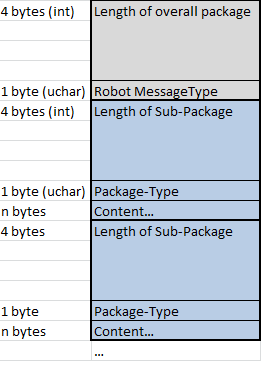
\includegraphics[width=0.5\textwidth]{pic/secondary_datapackage_scheme.png}
      \caption[Schema des Datenpackets gesendet von der Secondary Schnittstelle]{Grobe Darstellung wie das Nachrichten Packet gesendet von der Secondary/Primary Schnittstelle.}
      \label{fig:datascheme_of_secondary_interface}
\end{figure}

\subsection{Polyscope}
\label{urcontrol_polyscope_gru}

Polyscope ist eine Anwendung die auf dem Roboter-Rechner läuft. Die Anwendung verbindet sich per \acs{TCP/IP} auf den URControl(\ref{sec:ur_control_gru}) und sendet URScript befehler an den Roboter um diesen zu steuern.
Diese Anwendung wird auf dem Tablet angezeigt. Hierrüber kann man per Touch eingabe ein neues \acs{URP} Programm erstellen. Dieses Programm wird zur Laufzeit in ein Script umgewandelt. Die Polyscope Software schickt nun in Schritten die einzelnen Scriptbefehle an den URControl, der diese ausführt. Im Programmbaum kann eingesehen werden an welchem Schritt das Programm sich befindet.

\section{C-API}
\label{sec:rest_prinzip_gru}

Die C-\ac{API} ist von dem Hersteller \acs{UR} eine zur Verfügung gestellte C \acs{Library} mit einer Header Datei, die etwaige Funktionen der Library erklärt. Die Header Datei enthält nicht alle Funktionen, somit sind nicht alle zugänglich. Die C-\acs{API} erlaubt es einen eigenen Controller für den Roboter zu entwickeln. Der für den Roboter zur Verfügung gestellte Controller mit der Polyscope Software und eine anwendung die, die C-\acs{API} benutzt, kann aber nicht gleichzeitig laufen. Es schließen sich also die Programmiersprache URScript  und ein eigener Controller zunächst aus. Es könnte ein eigener Controller entwickelt werden, der die Befehle in URScript selbst interpretiert und diese wie bei dem URControll ausführt. So könnte man die vorhandene Sprache nehmen und diese sogar erweitern.

\subsection{Kontrollstruktur}
\label{capi_control_loop_gru}	

Die C-\acs{API} ermöglicht es eine Verbindung zum Roboter zu öffnen und über eigene Funktionen Befehle abzuschicken. Dies erfolgt in einem streng festgelegten Muster.

\begin{lstlisting}[language=C,caption={Beispiel der Kontroll Struktur}, label=lst:robot_control_loop,captionpos=b]
  while(!endcondition) { // At ROBOT_CONTROLLER_FREQUENCY times per second
    robotinterface_read_robot_state_blocking();
    robotinterface_get_actual_positions(&positions);
     // >>> various calculations <<<
    robotinterface_command_position_velocity_acceleration( xxx, yyy, zzz);
    robotinterface_send_robot_command();
  }
\end{lstlisting}

die Funktion robotinterface\_read\_state\_blocking() startet den Bereich in dem Datenabfragen an den Roboter gestellt werden können. Daten wie zb. Temperatur der Motoren, der Stand der Gelenke, die Geschwindigkeit der Gelenke, etc. in der Dokumentation beiliegend zu dieser Arbeit sind alle Daten noch einmal aufgelistet. Nachdem die Daten abgefragt wurden, kann mit C-\acs{API} Functionen Position, Geschwindigkeit und Beschleunigungswerte übermittelt werden, die der Roboter durch seinen Regler auszuführen versucht.\\
Es können jedoch keine Wegpunkte festgelegt werden, die dann automatisch vom Roboter angefahren werden. Dies muss der Entwickler selbst 
berechnen. Es gibt mehrere Verfahren, in dieser Arbeit sind \ac{PTP}-Verfahren und Linear Verfarhen(siehe Kapitel \ref{bewegungsprofile_gru}) getestet worden. In der beiliegenden Dokumentation ist aufgeführt wie man dies möglicherweise berwerkstelligen könnte.
\\\\
Zum Abschluss wird die Function robotinterface\_send() aufgerufen die dafür sorgt, dass der Acht Millisekundentakt eingehalten wird und die Befehle an den Roboter weiterleitet. Falls die Acht Millisekunden überschritten werden, wird der Roboter in einen Sicherheitsmodus gesetzt
und der Roboter wird angehalten.\\
Wenn so etwas im URController passiert, kann der Anwender diese wieder abschalten wenn alles in Ordnung ist. Dies muss mit der C-\acs{API} selbst geschrieben werden. Die C-\acs{API} liefert hierfür auch Funktionen. Das die richtigen Richtlinien aber auch eingehalten werden, muss von dem Wechsel des Sicherheitsmodus in den normalen Modus eine Benutzerabfrage verlangt werden.

\subsection{Bewegungsprofile}
\label{sub:bewegungsprofile_gru}

\acs{PTP} Verfahren 

Um den Roboter bestimmten Wegpunkten abfahren zu lassen, muss man die Bewegungsprofile selbst berechnen und ǘber die C-API an den Roboter im 125Hz Takt übergeben. Das \ac{PTP} Verfahren setzt dabei vorraus das die einzelnen Positionen der Gelenke bekannt sind. Der Wert ist angegeben in radiant. Die Zielposition

Linear Verfahren

Das Lineare Verfahren bedeutet eine Bewegung des Roboters von dem \ac{TCP} Punkt aus. Die Bewegung des Roboters wird so berechnet, dass der \acs{TCP} sich Linear zum Zielpunkt bewegt.(siehe Abbildung \ref{abbildung_linear})
Um die Berechnung durchzuführen muss die die Position des \acs{TCP} im Raum(Karthesische Koordinaten) bekannt sein, um eine Strecke zu einem Zielpunkt abfahren zu können. Der UR5 Roboter kann aber nur Positionen in Achs-Ebene verarbeiten. Deswegen muss zuerst eine Berechnung von Achs-Ebene in Karthesische Koordinaten und nach der Berechnung der Strecke wieder zurück auf Achs-Ebene erfolgen.

\section{Eigene Adapter Schnittstelle aufbauend auf URScript}
\label{sec:urscript_adapter}

Das Secondary Interface(\ref{urcontrol_spi_gru}) kann benutzt werden um einzelne Scriptbefehle an den Roboter zu senden. Auf diesem Prinzip aufbauend, kann ein Adapter für jede Programmiersprache entwickelt werden, der die Befehle an den Roboter sendet. Dadurch kann nun ein Anwendungsprogramm in dieser Sprache mit all seinen Vorteilen Entwickelt werden.

In dieser Arbeit wurde dafür Python gewählt. Gründe hierfür sind

\begin{itemize}
\item Weit verbreitete Programmiersprache
\item Ein vorhandener \acl{parsen} für die Secondary Schnittstelle
\item Viele vorhandene \acs{Software Bibliotheken}
\item Höhere Sprache als z.B C und somit etwas leichter zu Programmieren
\end{itemize}

Da aufbauend auf dieser Arbeit eventuell mit dem Roboter weitergearbeitet wird, wurde eine Sprache genommen die weit verbreitet ist. Python ist eine Sprache die nicht so Hardware nah ist, dass man sich um Speicherbelegung kümmern muss, aber den Code schnell ausführt.
Für den UR5 wurde eine \ac{ROS} Schnittstelle entwickelt, bei dem schon die Packete der Secondary Schnittstelle geparsed(\acl{parsen}) werden. Das Projekt ist öffentlich, so konnte dieser Code Abschnitt in die Arbeit übernommen werden.